\documentclass[12pt]{article}
\usepackage[top=.75in, bottom=.75in, left=.75in, right=.75in,portrait]{geometry}
\usepackage{amsmath}
\usepackage{amsfonts}
\usepackage{color}
\usepackage{graphicx}
\usepackage{subfig}
\renewcommand{\arraystretch}{1.5}
\usepackage{fancyhdr}
\pagestyle{fancy}
\renewcommand{\headrulewidth}{0pt}
\setlength\footskip{0pt}
\lhead{}
\rhead{}
\cfoot{}
\rfoot{08/13/2014}

\begin{document}

\section*{Error}
\begin{tabular}{| l | r |}
\hline
	No proliferation & 3.47 $\times 10^6$ \\ \hline
	With proliferation & 1.82 $\times 10^6$ \\ \hline
\end{tabular}

\vspace{2.5em}
\section*{Total Mass}
(calculated by adding up all the density values per pixel) \\
Blue: experimental data; \,\, Green: simulation; \qquad $x$-axis: frame \#

\begin{figure}[h!]
	\subfloat[No proliferation (mass conservation)]{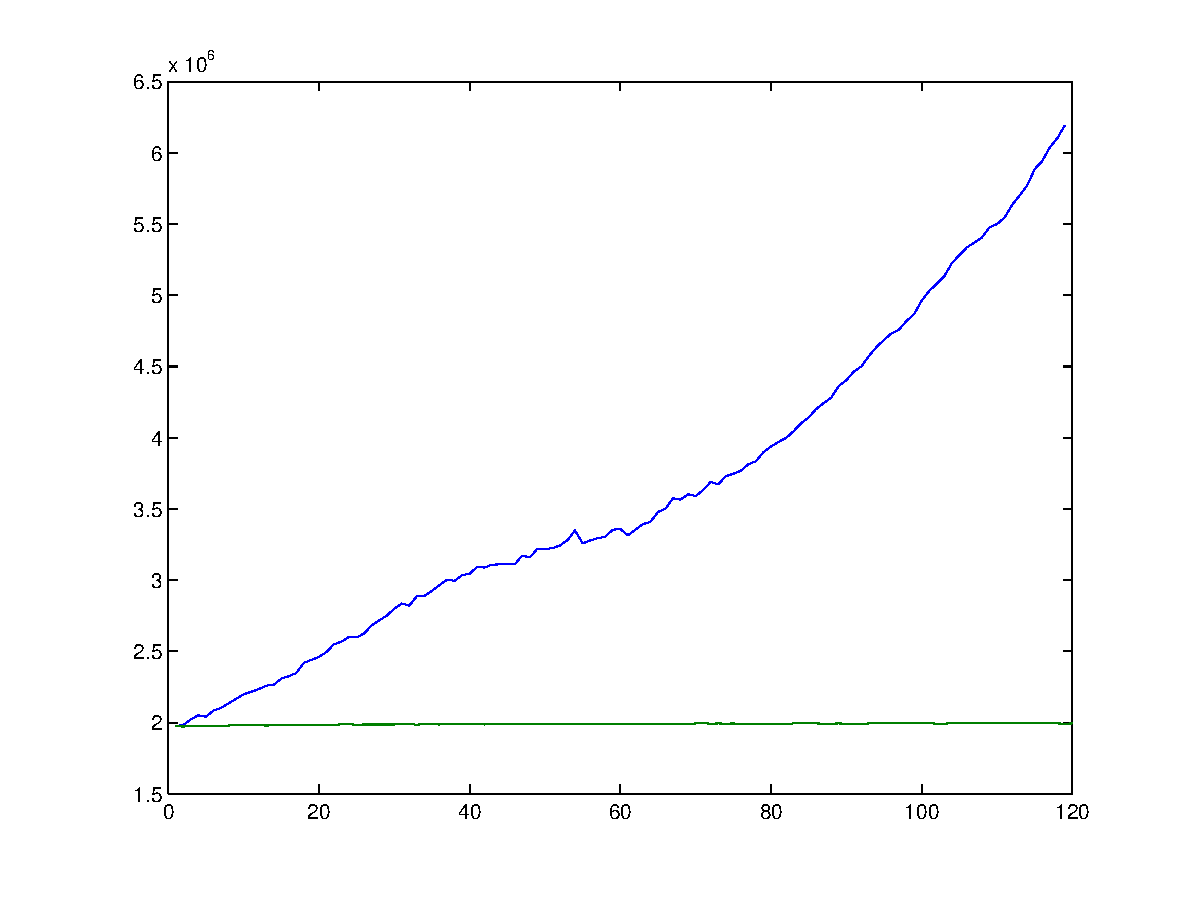
\includegraphics[width=.5\textwidth]{mass_Pos5_exp2_noprolif.eps}}
	\subfloat[With proliferation]{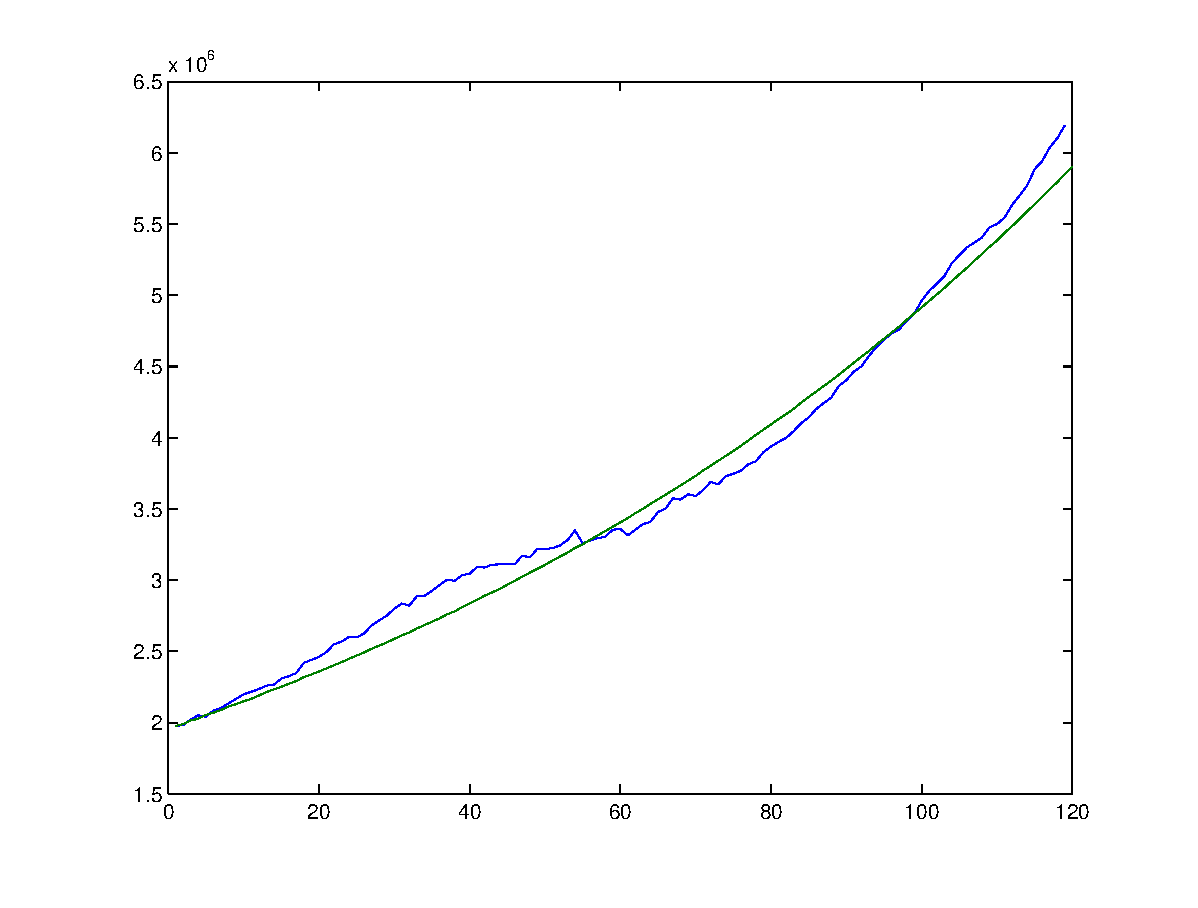
\includegraphics[width=.5\textwidth]{mass_Pos5_exp2_withprolif.eps}}
\end{figure}

\vspace{2.5em}
\section*{Boundaries}
\begin{figure}[h!]
	\subfloat[No proliferation]{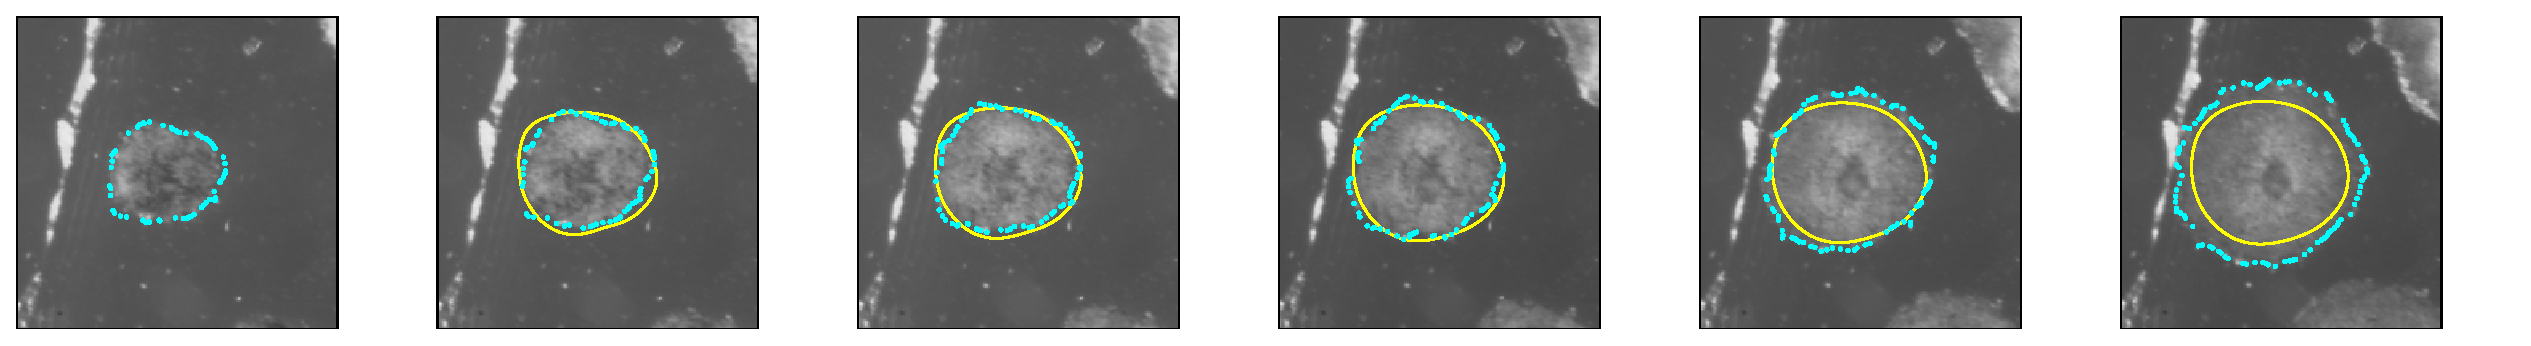
\includegraphics[width=\textwidth]{bdy_Pos5_exp2_noprolif.eps}} \\
	\subfloat[With proliferation]{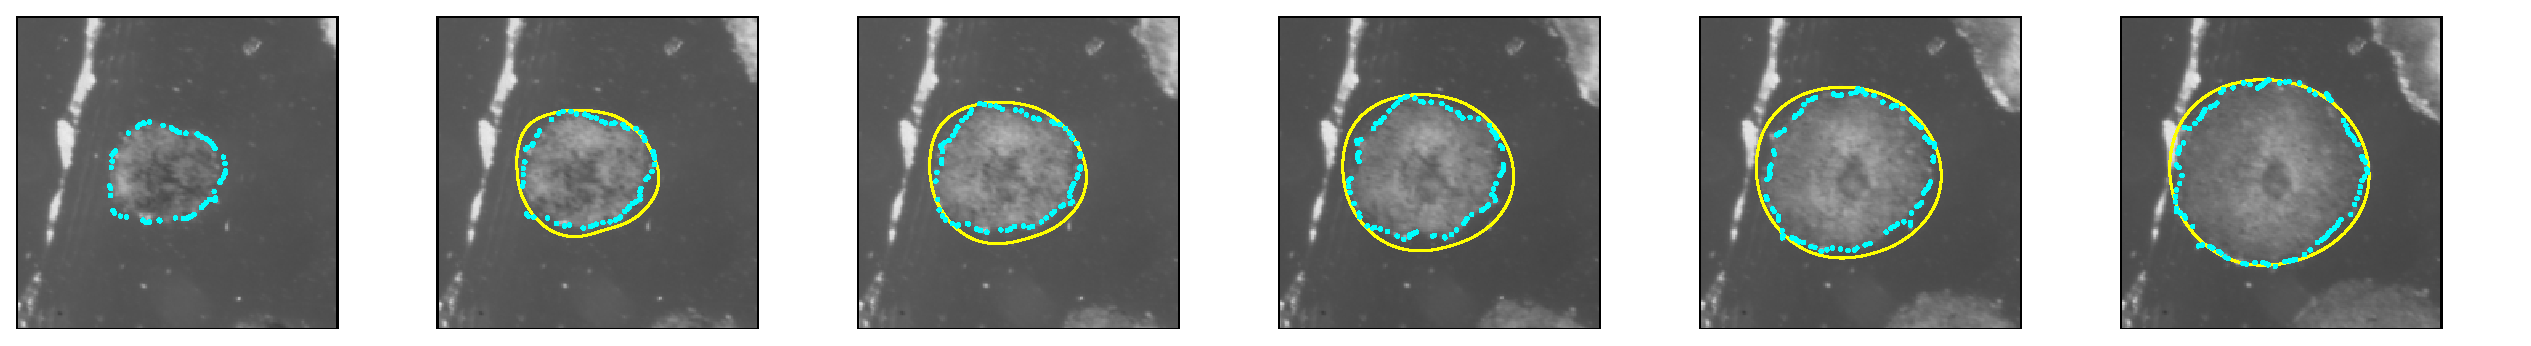
\includegraphics[width=\textwidth]{bdy_Pos5_exp2_withprolif.eps}}
\end{figure}


\section*{Densities}
\begin{figure}[h!]
	\subfloat[No proliferation]{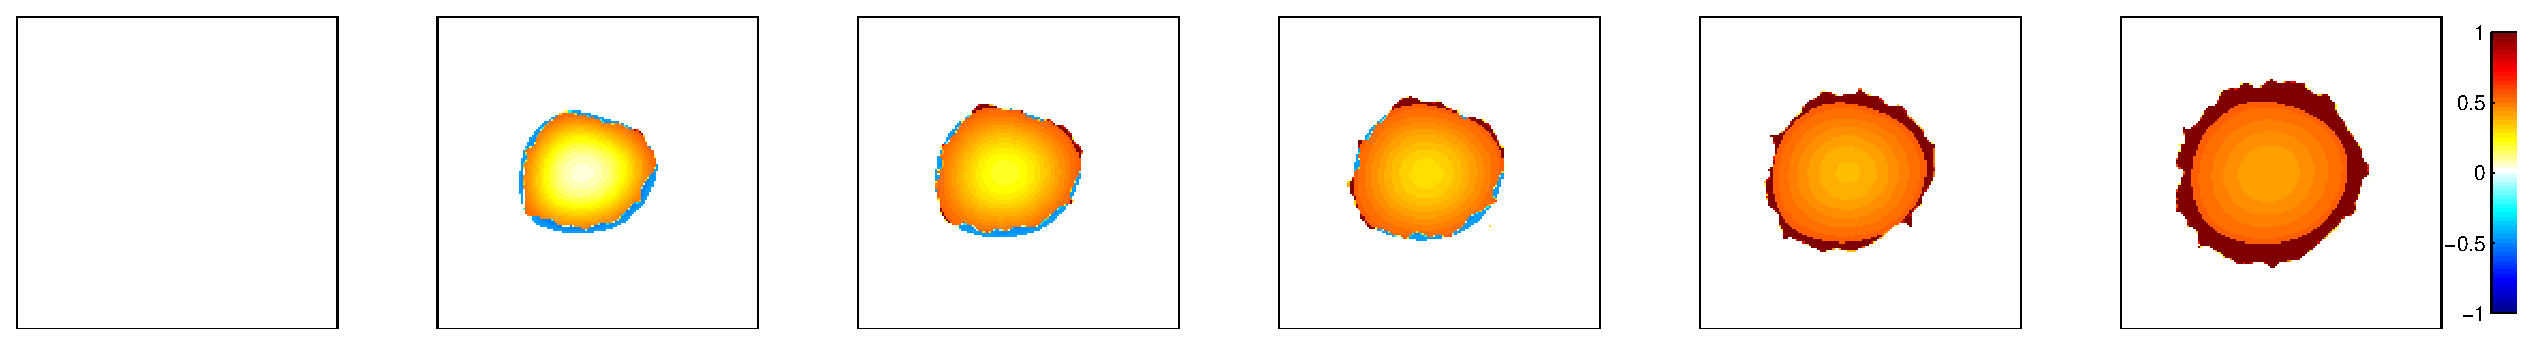
\includegraphics[width=\textwidth]{dens_Pos5_exp2_noprolif.eps}} \\
	\subfloat[With proliferation]{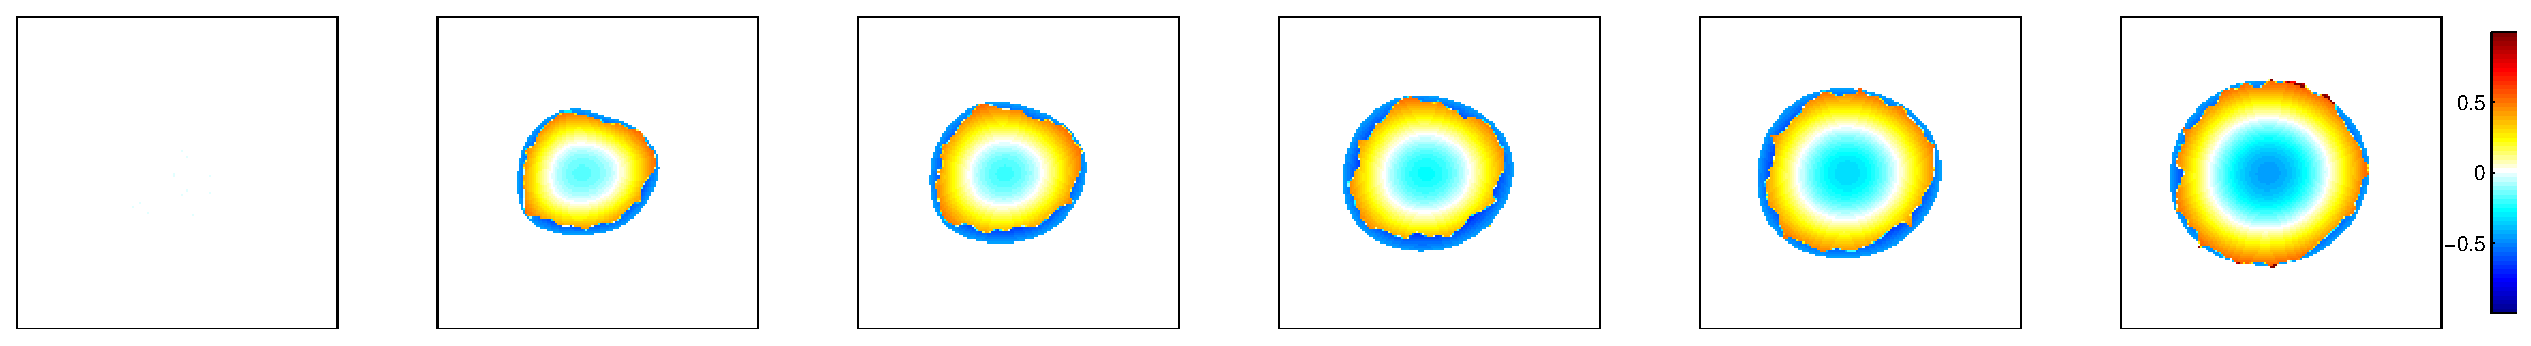
\includegraphics[width=\textwidth]{dens_Pos5_exp2_withprolif.eps}}
\end{figure}


\section*{Note}
Equation used for proliferation was $\frac{d \rho}{dt} = \frac{k}{b} \Delta \rho + \alpha \rho$ where $\alpha=0.11$.\\


I also tested having proliferation only occur where the cell colony was originally seeded, but this does not appear to give a better estimate ($\alpha=0.16$) -- Error: 2.38 $\times 10^6$

\begin{figure}[h!]
\centering
	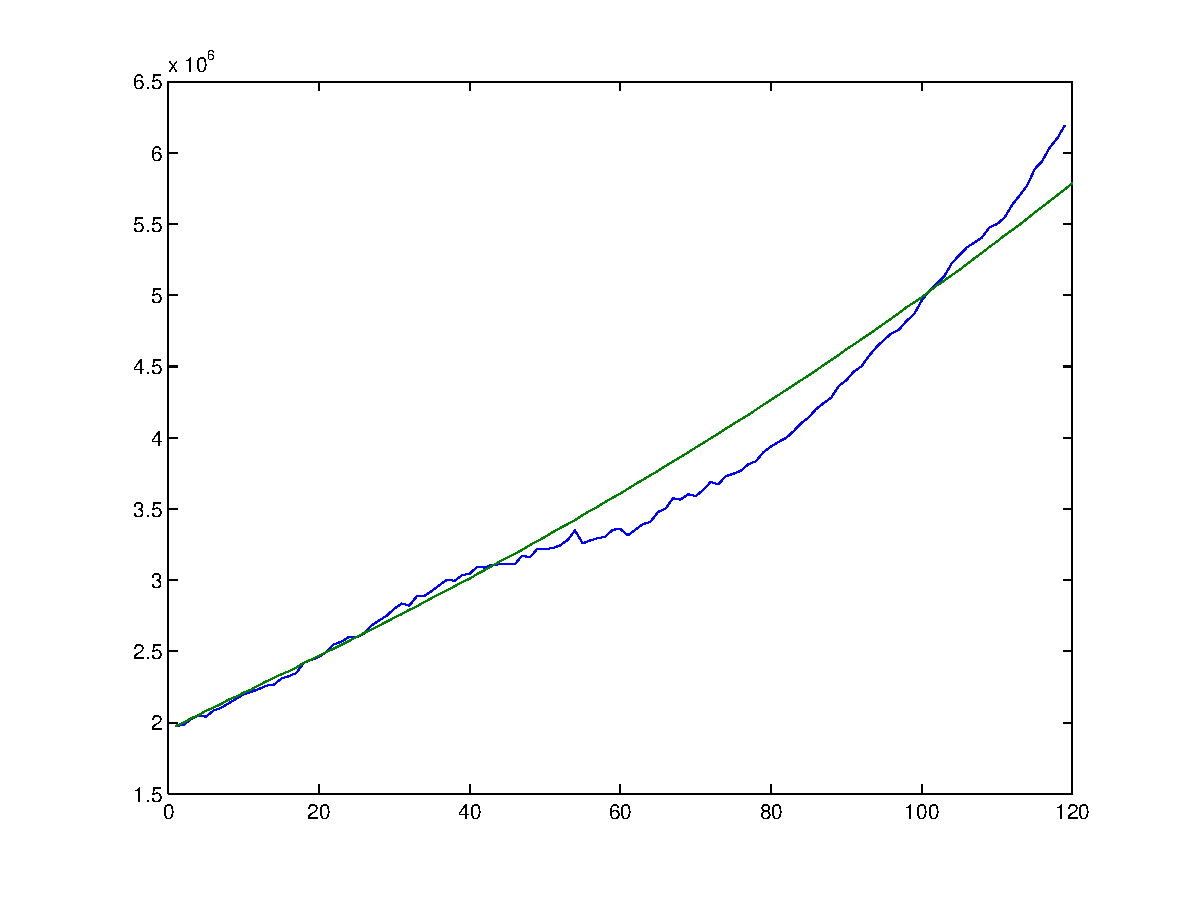
\includegraphics[width=.5\textwidth]{mass_Pos5_exp2_withprolif_onlyinorigloc.eps} \\
	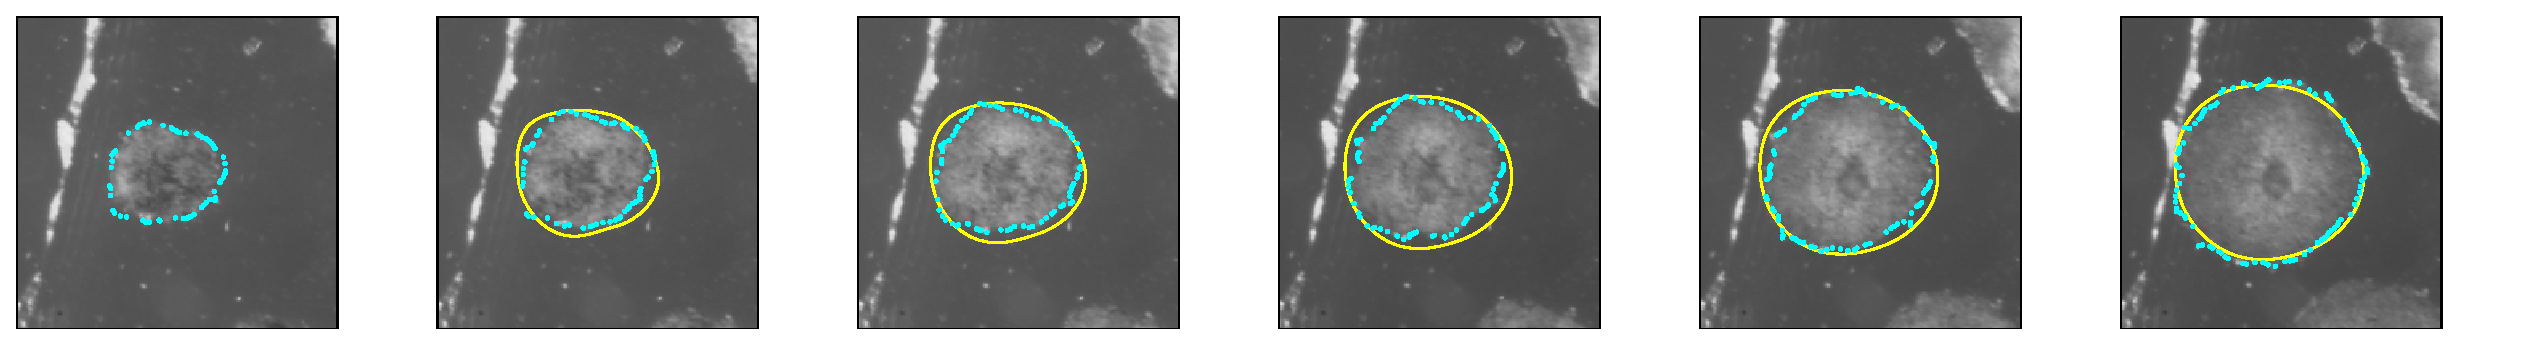
\includegraphics[width=\textwidth]{bdy_Pos5_exp2_withprolif_onlyinorigloc.eps} \\[.5em]
	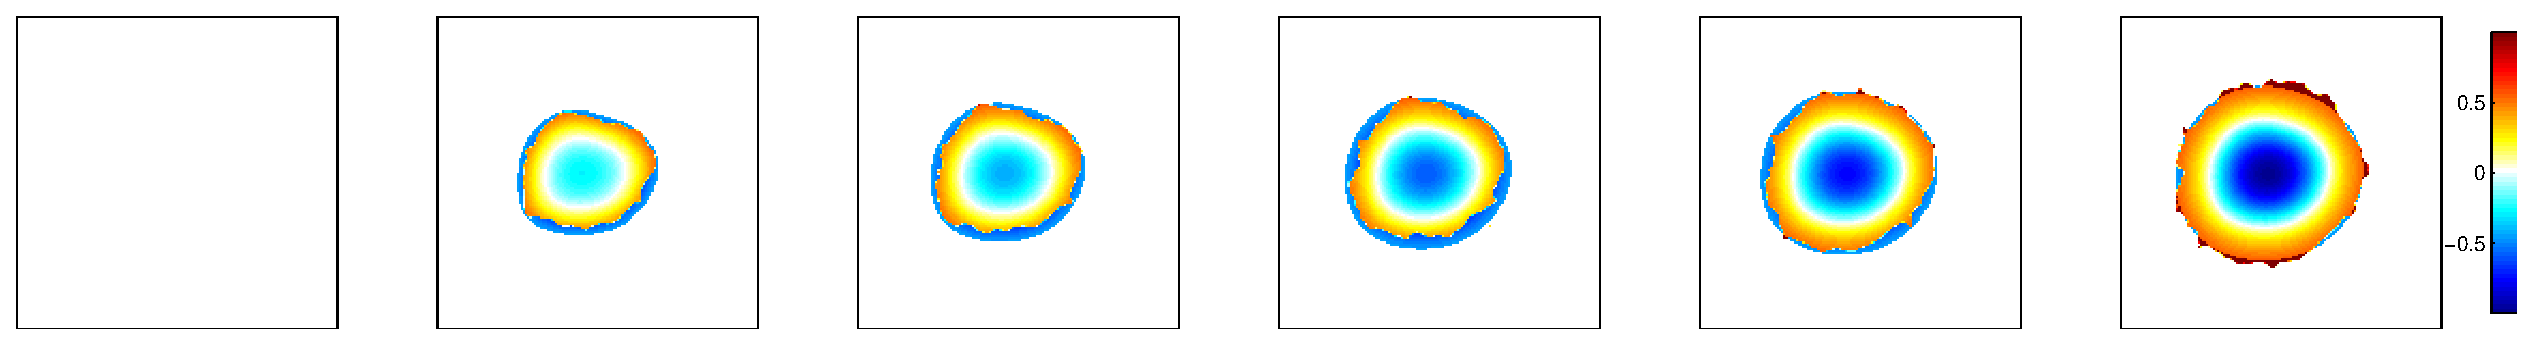
\includegraphics[width=\textwidth]{dens_Pos5_exp2_withprolif_onlyinorigloc.eps}
\end{figure}

\end{document}